\documentclass[a4paper,12pt]{article}

\usepackage{mystyle}

\usepackage{gensymb}
\usepackage{scalerel}
\usepackage{stackengine}

% \usepackage{skull}  % skull
\usepackage{halloweenmath}  % \bigpumpkin, skull (https://tug.ctan.org/info/symbols/comprehensive/symbols-a4.pdf -- Table 76)

\usepackage{tikzsymbols}

% https://tex.stackexchange.com/questions/3266/how-do-i-use-a-circle-as-a-math-accent-larger-than-mathring
% https://tex.stackexchange.com/a/3270/135045
\usepackage{accents}

\renewcommand{\mathring}[1]{\accentset{\circ}{#1}}


\graphicspath{ {images/} }


% https://tex.stackexchange.com/questions/5461/is-it-possible-to-change-the-size-of-an-arrowhead-in-tikz-pgf
\usetikzlibrary{arrows.meta}


\DeclareMathOperator{\Image}{Im}

\definecolor{pink}{RGB}{218, 3, 174}
\definecolor{violet}{RGB}{148, 0, 211}
\definecolor{green}{RGB}{0, 153, 0}
\definecolor{orange}{RGB}{255, 153, 0}
\definecolor{blue}{RGB}{5, 73, 255}
\definecolor{cyan}{RGB}{31, 206, 203}
\definecolor{cyan2}{RGB}{0, 166, 147}
\definecolor{cyangreen}{RGB}{0, 155, 118}
\definecolor{cyangreen2}{RGB}{0, 109, 91}


% https://tex.stackexchange.com/a/101138/135045

\newcommand\widesim[1]{\ThisStyle{%
  \setbox0=\hbox{$\SavedStyle#1$}%
  \stackengine{-.1\LMpt}{$\SavedStyle#1$}{%
    \stretchto{\scaleto{\SavedStyle\mkern.2mu\sim}{.5150\wd0}}{.6\ht0}%
  }{O}{c}{F}{T}{S}%
}}


\newcommand{\BigMiddleThree}{\;\left|\vphantom{\begin{pmatrix} 0\\0\\0 \end{pmatrix}}\right.\;}
\newcommand{\BigMiddleFour}{\;\left|\vphantom{\begin{pmatrix} 0\\0\\0\\0 \end{pmatrix}}\right.\;}


% https://tex.stackexchange.com/questions/63531/how-to-write-quotation-marks-in-math-environment
\DeclareMathSymbol{\mlq}{\mathord}{operators}{``}
\DeclareMathSymbol{\mrq}{\mathord}{operators}{`'}


\DeclareMathOperator{\Imag}{Im}


% https://tex.stackexchange.com/questions/544453/undefined-control-sequence-after-paragraph
\renewcommand{\paragraph}[1]{\noindent\textbf{#1}\quad}


% https://tex.stackexchange.com/questions/36851/skipping-line-after-proof-in-proof-environment#comment73553_36851
\newcommand{\proofindent}{\hspace*{\fill}\par\vspace{0.5em}\noindent}


% https://tex.stackexchange.com/questions/4813/extendible-equals-sign
\makeatletter
\newcommand*{\Relbarfill@}{\arrowfill@\Relbar\Relbar\Relbar}
\newcommand*{\xeq}[2][]{\ext@arrow 0055\Relbarfill@{#1}{#2}}
\makeatother


% https://tex.stackexchange.com/questions/279100/typeset-the-shrug-%C2%AF-%E3%83%84-%C2%AF-emoji
\newcommand{\shrug}[1][]{%
\begin{tikzpicture}[baseline,x=0.8\ht\strutbox,y=0.8\ht\strutbox,line width=0.125ex,#1]
  \def\arm{(-2.5,0.95) to (-2,0.95) (-1.9,1) to (-1.5,0) (-1.35,0) to (-0.8,0)};
  \draw \arm;
  \draw[xscale=-1] \arm;
  \def\headpart{(0.6,0) arc[start angle=-40, end angle=40,x radius=0.6,y radius=0.8]};
  \draw \headpart;
  \draw[xscale=-1] \headpart;
  \def\eye{(-0.075,0.15) .. controls (0.02,0) .. (0.075,-0.15)};
  \draw[shift={(-0.3,0.8)}] \eye;
  \draw[shift={(0,0.85)}] \eye;
  % draw mouth
  \draw (-0.1,0.2) to [out=15,in=-100] (0.4,0.95); 
\end{tikzpicture}}



% https://tex.stackexchange.com/a/314638/135045
% \newcommand{\diff}{\mathop{}\!d\!}
\newcommand{\diff}{\mathop{}\!d}


\author{Алексеев Василий}


\title{Семинар 9}
\date{11 ноября 2024}


\begin{document}
  \maketitle
  
  \tableofcontents

  \thispagestyle{empty}
  
  \newpage
  
  
  
  \vspace*{\fill}
  
  \noindent
  \emph{
    К формулировкам и доказательствам (если такие вообще приводятся) стоит относиться критически.
    Основное в этом конспекте~---~решение задач (но ``критичность'' и здесь лучше не отключать).
    За строгой, ясной и последовательной теорией лучше обращаться к ``нормальным'' источникам.
    (Например, к лекциям.)
  }
  
  \vspace*{\fill}
  
  \thispagestyle{empty}
  
  \newpage
  
  
  \pagenumbering{arabic}


  \section{Формула Тейлора}
  
  %\begin{figure}[ht]
    %\centering
    %\includegraphics[width=0.6\linewidth]{images/Apples}
    %
    %\caption{
      %Одно яблоко, два яблока, ...~---~натуральные числа используются при счёте предметов.
    %}
    %\label{fig:naturals}
  %\end{figure}
  
  
  % [X] физический типа вывод
  % [X] основные функции
  % [X] неопределённые коэффициенты
  % [X] от производной
  % [X] примеры с картинки


  \subsection{Сюжет из физики}

  Пусть материальная точка движется вдоль оси~$X$ с постоянным ускорением~$a(t) \hm= \text{const}$.
  В таком случае, если начальная скорость была равна~$v_0$, то скорость в произвольный момент времени~$v(t)$ можно рассчитать следующим образом:\footnote{
    Под ускорением~$a(t)$ и скоростью~$v(t)$ в данном случае понимаются проекции соответствующих векторов на ось~$X$: $a \hm\equiv a_x$, $v \hm\equiv v_x$.
  }
  \begin{equation*}
  \begin{split}
    a(t) = \frac{\diff v(t)}{\diff t} &\Rightarrow \diff v(t) = a(t) \diff t\\
    &\Rightarrow \int_0^t v(\tau) = \int_0^t a(\tau) \diff \tau\\
    &\Rightarrow v(t) = v_0 + a t
  \end{split}
  \end{equation*}

  Если начальная координата была равна~$x_0$, то координату в зависимости от времени~$x(t)$ тоже можно найти~---~из аналогичных рассуждений:
  \begin{equation*}
  \begin{split}
    v(t) = \frac{\diff x(t)}{\diff t} &\Rightarrow \diff x(t) = v(t) \diff t\\
    &\Rightarrow \int_0^t x(\tau) = \int_0^t v(\tau) \diff \tau\\
    &\Rightarrow \int_0^t x(\tau) = \int_0^t (v_0 + a \tau) \diff \tau\\
    &\Rightarrow x(t) = x_0 + v_0 t + \frac{at^2}{2}
  \end{split}
  \end{equation*}

  Учитывая, что
  \[
    \begin{aligned}
      &v(t) = x'(t)\\
      &a(t) = x''(t)
    \end{aligned}
  \]
  соотношение для определения координаты~$x(t)$ можно переписать так:
  \[
    x(t) = x(0) + x'(0) t + \frac{x''(0)}{2}t^2
  \]

  Если бы ускорение было переменным и была бы известна его скорость изменения, то в формуле возник бы член с~$t^3$, и так далее.
  Но даже если бы ускорение было переменным, формулой выше (до $t^2$) можно бы было пользоваться~---~только надо бы было понимать, что эта формула будет тем точнее, чем \emph{ближе} рассматриваемое время~$t$ к нулевому моменту времени.
  Это~---~пример формулы Тейлора для функции~$x(t)$ в окрестности нуля (формула Маклорена).

  Общий вид формулы Тейлора для некоторой функции~$f(x)$ в окрестности точки~$x_0$:\footnote{
    Точнее, это формула Тейлора \emph{с остаточным членом в форме Пеано}.
    Для существования такого разложения функция должна быть определена в некоторой окрестности точки~$x_0$, должна иметь в окрестности~$x_0$ производные до $(n \hm- 1)$-го порядка включительно, а в самой~$x_0$ должна существовать и $n$-ая производная.
  }
  \[
    f(x) = f(x_0) + f'(x_0) \cdot (x - x_0) + \frac{f''(x_0)}{2} \cdot (x - x_0)^2 + \ldots + \frac{f^{(n)}(x_0)}{n!} \cdot (x - x_0)^n + o((x - x_0)^n),\ x \to x_0
  \]
  \begin{equation}
    f(x) = \sum_{k = 0}^n \frac{f^{(k)}(x_0)}{k!} (x - x_0)^k + o((x - x_0)^n),\ x \to x_0
  \end{equation}

  И частный её случай~---~формула Маклорена (представление функции~$f$ в окрестности нуля: $x_0 \hm= 0$):
  \[
    f(x) = f(0) + f'(0) \cdot x + \frac{f''(0)}{2} \cdot x^2 + \ldots + \frac{f^{(n)}(0)}{n!} \cdot x^n + o(x^n),\ x \to 0
  \]
  \begin{equation}\label{eq:maclore}
    f(x) = \sum_{k = 0}^n \frac{f^{(k)}(0)}{k!} x^k + o(x^n),\ x \to 0
  \end{equation}


  \subsection{Некоторые ``табличные'' формулы Маклорена}

  Просто вычислением $n$-ых производных в нуле можно получить формулы Маклорена следующих функций.

  Экспонента:
  \[
    e^x = 1 + x + \frac{x^2}{2} + \frac{x^3}{3!} + \ldots
  \]
  \begin{equation}\label{eq:exp}
    e^x = \sum_{k = 0}^n \frac{x^k}{k!} + o(x^n),\ x \to 0
  \end{equation}

  Гиперболический синус (``шинус''):\footnote{
    Как у нечётной функции: $f(-x) \hm= -f(x)$,~---~в формуле Тейлора будут присутствовать члены только с~$x$ в \emph{нечётной} степени.
    Иначе, если всё-таки допустить наличие ненулевого члена с чётной степенью: $f(x) \hm= \ldots \hm+ C x^{2k} \hm+ \ldots$,~---~то получим противоречие:
    \[
      f(-x) = \ldots + C x^{2k} + \ldots \not= -\ldots - C x^{2k} - \ldots = -f(x)
    \]
  }
  \[
    \sh x = x + \frac{x^3}{3!} + \frac{x^5}{5!} + \ldots
  \]
  \begin{equation}\label{eq:sh}
    \sh x = \sum_{k = 0}^n \frac{x^{2k + 1}}{(2k + 1)!} + o(x^{2n + 2}),\ x \to 0
  \end{equation}

  Гиперболический косинус (``чосинус''):\footnote{
    Как у чётной функции: $f(-x) \hm= f(x)$,~---~в формуле Тейлора будут только члены с~$x$ в \emph{чётной} степени.
  }
  \[
    \ch x = 1 + \frac{x^2}{2} + \frac{x^4}{4!} + \ldots
  \]
  \begin{equation}\label{eq:ch}
    \ch x = \sum_{k = 0}^n \frac{x^{2k}}{(2k)!} + o(x^{2n + 1}),\ x \to 0
  \end{equation}

  Просто синус:
  \[
    \sin x = x - \frac{x^3}{3!} + \frac{x^5}{5!} - \ldots
  \]
  \begin{equation}\label{eq:sin}
    \sin x = \sum_{k = 0}^n (-1)^{k} \frac{x^{2k + 1}}{(2k + 1)!} + o(x^{2n + 2}),\ x \to 0
  \end{equation}

  Просто косинус:
  \[
    \cos x = 1 - \frac{x^2}{2} + \frac{x^4}{4!} - \ldots
  \]
  \begin{equation}\label{eq:cos}
    \cos x = \sum_{k = 0}^n (-1)^k \frac{x^{2k}}{(2k)!} + o(x^{2n + 1}),\ x \to 0
  \end{equation}

  Для полноты картины\footnote{
    А также потому, что это может пригодиться при решении задач на пределы...
  } приведём ещё ``кусочки'' (только первые члены) формул Тейлора для тангенса, арксинуса и арктангенса (и также вспомним в начале ещё синус для сравнения):\footnote{
    Кусочки, а не полные формулы~---~потому, что составление формулы Тейлора через вычисление производной $n$-ого порядка в данных случаях кажется проблематичным...
  }\textsuperscript{,}\footnote{  % TODO: ``аркшинус'', ``аркщангенс'' (?)
    При этом можно иметь в виду, что:
    \[
      \begin{aligned}
        &\arccos x = \frac{\pi}{2} - \arcsin x\\
        &\arcctg x = \frac{\pi}{2} - \arctg x
      \end{aligned}
    \]
  }
  \[
    \sin x = x - \frac{x^3}{6} + o(x^4)
  \]
  \begin{equation}\label{eq:easy-tg}
    \tg x = x + \frac{x^3}{3} + o(x^4)
  \end{equation}
  \begin{equation}\label{eq:easy-arcsin}
    \arcsin x = x + \frac{x^3}{6} + o(x^4)
  \end{equation}
  \begin{equation}\label{eq:easy-arctg}
    \arctg x = x - \frac{x^3}{3} + o(x^4)
  \end{equation}

  ``Скобка'' ($\alpha \in \RR$):\footnote{
    Далее в формуле используется следующее (``продвинутое'') обозначение для биномиального коэффициента (``цэ из эн по ка''):
    \[
      \binom{\alpha}{k} = C_{\alpha}^k
    \]
  }
  \[
    (1 + x)^{\alpha} = 1 + \alpha x + \frac{\alpha (\alpha - 1)}{2} x^2 + \ldots
  \]
  \begin{equation}\label{eq:brace}
    (1 + x)^{\alpha} = \sum_{k = 0}^n \binom{\alpha}{k} x^k + o(x^n)
  \end{equation}

  \begin{example}
    Приведём также пару популярных частных случаев ``скобки''.

    Случай один:
    \[
      \frac{1}{1 + x} = (1 + x)^{-1} = 1 - x + \frac{-1(-2)}{2} x^2 + \frac{-1(-2)(-3)}{3!} x^3 + \ldots
    \]
    \begin{equation}\label{eq:1-div-plus}
      \frac{1}{1 + x} = 1 - x + x^2 - x^3 + \ldots
    \end{equation}

    Случай два:
    \[
      \frac{1}{1 - x} = (1 - x)^{-1} = (1 + (-x))^{-1} = 1 - (-x) + \frac{-1(-2)}{2} (-x)^2 + \frac{-1(-2)(-3)}{3!} (-x)^3 + \ldots
    \]
    \begin{equation}\label{eq:1-div-minus}
      \frac{1}{1 - x} = 1 + x + x^2 + x^3 + \ldots
    \end{equation}
  \end{example}

  И формула для логарифма:\footnote{
    Получить её можно либо тоже ``стандартно'': нахождением $n$-ой производной.
    Либо через ``трюк'' с производной (через формулу Тейлора для производной)~---~пример про это см. далее~(\ref{p:T5}).
  }
  \[
    \ln{(1 + x)} = x - \frac{x^2}{2} + \frac{x^3}{3} - \ldots
  \]
  \begin{equation}\label{eq:log-plus}
    \ln{(1 + x)} = \sum_{k = 1}^n (-1)^{k - 1} \frac{x^k}{k} + o(x^n)
  \end{equation}

  И ещё одна:
  \[
    \ln{(1 - x)} = \ln{(1 + (-x))} = -x - \frac{(-x)^2}{2} + \frac{(-x)^3}{3} - \ldots
  \]
  \begin{equation}\label{eq:log-minus}
    \ln{(1 - x)} = \sum_{k = 1}^n - \frac{x^k}{k} + o(x^n)
  \end{equation}

  
  \subsection{С1, \S 9, \textnumero 50(1)}
  
  Установить, какое из утверждений верно:
  \begin{itemize}
    \item[a)] $x^2 = o(x),\quad x \to 0$
    \item[b)] $x^2 = o(x),\quad x \to \infty$
  \end{itemize}
  
  \begin{solution}
    Что означает выражение $x^2 \hm= o(x)$?
    Оно говорит о том, что $x^2$ ``бесконечно'' мал по сравнению с $x$.
    Если $x \hm\approx 0$ ($x \hm\to 0$), то $x^2$ будет намного меньше, чем~$x$.
    Если же $x \hm\gg 1$ ($x \hm\to \infty$), то $x^2$, наоборот, будет намного больше, чем просто~$x$.
    Итого:
    \[
      \begin{aligned}
        &x^2 = o(x),\quad x \to 0\\
        &x = o(x^2),\quad x \to \infty
      \end{aligned}
    \]
    
    И более ``формально строгое'' обоснование:
    \[
      \lim_{x \to 0} \frac{x^2}{x} = \lim_{x \to 0} x = 0 \quad\Rightarrow\quad x^2 = o(x),\quad x \to 0
    \]
  \end{solution}
  
  
  
  \subsection{С1, \S 9, \textnumero 51(2)}
  
  Показать, что
  \[
    o(x^n) \cdot o(x^k) = o(x^{n + k}),\quad x \to 0
  \]
  (где $n, k \in \NN$).
  
  \begin{solution}
    Доказываемое равенство~---~между классами функций.
    Функция ``слева''~---~это произведение некоторых двух $f(x)$ и $g(x)$, про каждую из которых известно, что:
    \[
      \lim_{x \to 0} \frac{f(x)}{x^n} = 0,\quad \lim_{x \to 0} \frac{g(x)}{x^k} = 0
    \]
    
    Проверим, лежит ли эта функция~--~произведение двух в классе $o(x^{n + k})$ при $x \hm\to 0$:
    \[
      \lim_{x \to 0} \frac{f(x) \cdot g(x)}{x^{n + k}} = \lim_{x \to 0} \frac{f(x)}{x^n} \cdot \frac{g(x)}{x^k} = 0
        \quad\Rightarrow\quad (fg)(x) = o(x^{n + k}),\ x \hm\to 0
    \]
  \end{solution}

  
  
  Перед следующим номером рассмотрим сначала небольшой
  
  \begin{example}
    \[
      \bigl(x + o(x)\bigr) + \bigl(x^2 + o(x^2)\bigr) = x + o(x),\ x \to 0
    \]
  \end{example}
  
  
  
  \subsection{Т4}
  
  Упростить выражение:
  \[
    (2x - 3x^4 + o(x^4)) \cdot (1 - x + 2x - x^3 + o(x^3))
  \]
  
  \begin{solution}
    Иными словами, считаем, что упростить надо такое выражение:
    \[
      (2x - 3x^4 + o(x^4)) \cdot (1 + x - x^3 + o(x^3))
    \]
    
    Можно по-честному раскрыть скобки и потом ``спрятать'' в о-малое всё лишнее.
    А можно попытаться сразу прикинуть, до какой точности имеет вообще смысл проводить вычисления.
    Какая получится ``самая большая'' о-малая в результате раскрытия скобок?
    Видно, что это $o(x^4)$ (так как $o(x^4) \hm\cdot 1 \hm= o(x^4)$ и $o(x^3) \hm\cdot 2x \hm= o(x^4)$).
    Таким образом, все слагаемые с $x$ в степени~$5$ и выше нам ``не интересны''.
    А для всех $x$ в меньших степенях можем собрать коэффициенты в виде суммы.
    В результате такого ``интеллектуального'' раскрытия скобок получаем:
    \[
      0 \cdot 1 + 2 \cdot x + 2 \cdot x^2 + 0 \cdot x^3 + (-3 - 2) \cdot x^4 + o(x^4)
        = 2x + 2x^2 - 5x^4 + o(x^4),\ x \to 0
    \]
  \end{solution}
  
  
  
  %%%%%%%
  %%% Новый семинар
  %%%%%%%
  
  
  \subsection{С1, \S 18, \textnumero 1(9)}
  
  Представить формулой Маклорена до $o(x^n)$ функцию:
  \[
    f(x) = \frac{1}{(1 - x)^2}
  \]
  
  \begin{solution}
    Выражение, задающее функцию, имеет вид $(1 + x)^{\alpha}$:
    \[
      f(x) = (1 - x)^{-2}
    \]
    
    Поэтому по~\eqref{eq:brace} в качестве формулы Маклорена получаем:
    \[
      f(x) = (1 - x)^{-2} = 1 + (-2) \cdot (-x) + \frac{(-2) \cdot (-2 - 1)}{2} \cdot (-x)^2 + \ldots + \binom{-2}{n} (-x)^n + o(x^n),\ x \to 0
    \]
    
    Для полноты картины можем попробовать получить числовое выражение для $n$-ого коэффициента:
    \begin{equation*}
    \begin{split}
      \binom{-2}{k} &= \frac{-2 \cdot (-2 - 1) \cdot \ldots \cdot (-2 - (k - 1))}{k!}\\
        &= (-1)^k \cdot \frac{2 \cdot 3 \cdot \ldots \cdot (k + 1)}{k!}\\
        &= (-1)^k \frac{(k + 1)!}{k!} = (-1)^k \cdot (k + 1)
    \end{split}
    \end{equation*}
    
    Итого:
    \[
      f(x) = \sum_{k = 0}^n (-1)^k (k + 1) \cdot (-1)^k x^k + o(x^n)
        = \sum_{k = 0}^n (k + 1) \cdot x^k + o(x^n)
    \]
  \end{solution}
  
  
  
  
  \subsection{С1, \S 18, \textnumero 2(9)}
  \label{n:1-18-2(9)}
  
  Представить формулой Маклорена до $o(x^n)$ функцию:
  \[
    f(x) = \ln{(2 + x - x^2)}
  \]
  
  \begin{solution}
    Так как $x \hm- x^2 \hm\to 0$ при $x \hm\to 0$, то можно попробовать сразу воспользоваться формулой Тейлора для логарифма~\eqref{eq:log-plus}:
    \begin{equation*}
    \begin{split}
      \ln{(2 + x - x^2)} &= \ln 2 + \ln\left(1 + \frac{x - x^2}{2}\right)\\
        &= \ln 2 + \frac{x - x^2}{2} - \frac{1}{2} \cdot \left(\frac{x - x^2}{2}\right)^2 + \frac{1}{3} \cdot \left(\frac{x - x^2}{2}\right)^3 - \ldots\\
        &= \ln 2 + \frac{1}{2} x + \left(-\frac{1}{2} - \frac{1}{8}\right) x^2 + o(x^2)
    \end{split}
    \end{equation*}
    
    Видно, что разложение до какого-то фиксированного небольшого числа членов таким образом получить можно, но общую формулу до $n$-ого члена~---~уже как-то затруднительно...
    Поэтому придётся пойти другим путём.
    
    Заметим, что выражение под логагифмом несложным образом раскладывается на множители:
    \[
      2 + x - x^2 = -(x^2 - x - 2) = -(x + 1)(x - 2)
    \]
    
    Поэтому функцию в окрестности нуля можно представить таким образом:\footnote{
      Модулей при разложении одного логарифма в сумму двух нигде не ставим, потому что осознанно контролируем, чтоб выражения под логарифмами были положительными~---~в близкой окрестности нуля.
    }
    \[
      f(x) = \ln{\bigl\{-(x + 1)(x - 2)\bigr\}} = \ln{\bigl\{(1 + x)(2 - x)\bigr\}} = \ln{(1 + x)} + \ln{(2 - x)}
    \]
    
    % https://tex.stackexchange.com/questions/51195/multiple-items-equations-in-single-eqref-call
    Теперь уже понятно~(\ref{eq:log-plus},~\ref{eq:log-minus}), что делать дальше:
    \[
      \ln{(1 + x)} = x - \frac{x^2}{2} + \frac{x^3}{3} + \ldots = \sum_{k = 1}^n (-1)^{k - 1} \frac{x^k}{k} + o(x^n),\ x \to 0
    \]
    \begin{equation*}
    \begin{split}
      \ln{(2 - x)} &= \ln 2 + \ln\left(1 - \frac{x}{2}\right)\\
      &= \ln 2 - \frac{x}{2} - \frac{1}{2} \cdot \left(\frac{x}{2}\right)^2 - \frac{1}{3} \cdot \left(\frac{x}{2}\right)^3 - \ldots\\
      &= \ln 2 - \sum_{k = 1}^n \frac{1}{k} \left(\frac{x}{2}\right)^k + o(x^n),\ x \to 0
    \end{split}
    \end{equation*}
    
    (Замечаем, что до $o(x^2)$ таким образом полученное разложение $f(x)$ будет совпадать с первоначальным вариантом через логарифм в лоб.)
    
    Итого:
    \[
      f(x) = \ln 2 + \sum_{k = 1}^n \frac{1}{k} \cdot \left((-1)^{k - 1} - \left(\frac{1}{2}\right)^k\right) \cdot x^k + o(x^n),\ x \to 0
    \]
  \end{solution}
  
  
  
  \subsection{С1, \S 18, \textnumero 3(4)}
  
  Представить формулой Маклорена до $o(x^n)$ функцию:
  \[
    f(x) = x \sqrt[3]{4 - 4x + x^2}
  \]
  
  \begin{solution}
    Как и в номере~\ref{n:1-18-2(9)}, корень вообще можно бы было разложить да какого-то члена сразу, имея в виду, что $-4x \hm+ x^2 \hm\to 0$ при $x \hm\to 0$, но красивой формулы до произвольного $n$-ого члена таким образом, скорее всего, также не получится...
    
    Поэтому, аналогично тому, как было сделано в упомянутом номере, заметим, что подкоренное выражение раскладывается на... представляет из себя полный квадрат:
    \[
      4 - 4x + x^2 = x^2 - 4x + 4 = (x - 2)^2
    \]
    
    Таким образом, функция выглядит так:
    \[
      f(x) = x (x - 2)^{2/3} = 2^{2/3} \cdot x \cdot (1 - x/2)^{2/3}
    \]
    
    И её разложение в формулу Тейлора~\eqref{eq:brace}:\footnote{
      Получить ``красивую'' формулу для коэффициента $\binom{2/3}{k}$ у автора конспекта не получилось.
    }
    \begin{equation*}
    \begin{split}
      f(x) &= 2^{2/3} \cdot x \cdot \left(1 - \frac{2}{3} \cdot \frac{x}{2} + \frac{(2/3)(2/3 - 1)}{2} \left(-\frac{x}{2}\right)^2 + \ldots\right)\\
        &= 2^{2/3} \cdot x \cdot \left(\sum_{k = 0}^n \binom{2/3}{k} \left(-\frac{x}{2}\right)^k + o(x^n)\right)\\
        &= \sum_{k = 0}^n (-1)^k \cdot 2^{2/3 - k} \cdot \binom{2/3}{k} \cdot x^{k + 1} + o(x^{n + 1})
    \end{split}
    \end{equation*}
  \end{solution}
  
  
  
  \subsection{С1, \S 18, \textnumero 14(2)}
  
  Представить формулой Тейлора в окрестности точки~$x_0$ до $o((x \hm- x_0)^n)$ функцию:
  \[
    f(x) = \ln{\sqrt[4]{\frac{x - 2}{5 - x}}},\ x_0 = 3
  \]
  
  \begin{solution}
    Сделаем замену:
    \[
      \begin{aligned}
        &t \equiv x - x_0 = x - 3 & &\leftrightarrow & &x = t + 3\\
        &x \to x_0 & &\leftrightarrow & &t \to 0
      \end{aligned}
    \]
    
    Тогда функция:\footnote{
      Вообще это будет уже новая функция $\phi(t) \hm\equiv f\bigl(x(t)\bigr)$ (новое правило расчёта зависимой переменной по независимой), но для простоты обозначим её так же: $f(t)$.
    }
    \[
      f(t) = \ln{\sqrt[4]{\frac{t + 3 - 2}{5 - t - 3}}}
        = \ln{\sqrt[4]{\frac{t + 1}{2 - t}}}
    \]
    
    И преобразуем, чтобы прийти к ``табличным'' формулам Тейлора:\footnote{
      Модулей при разложении логарифма таким образом в сумму не возникает.
    }
    \begin{equation*}
    \begin{split}
      f(t) &= \frac{1}{4} \cdot \left\{
        \ln{(1 + t)} - \ln{(2 - t)}
      \right\}\\
      &= \frac{1}{4} \cdot \left\{
        \sum_{k = 1}^n (-1)^{k - 1} \frac{t^k}{k} - \ln 2 - \sum_{k = 1}^n (-1)^{k - 1} \frac{(t/2)^k}{k} + o(t^n)
      \right\}\\
      &= -\frac{\ln 2}{4} + \sum_{k = 1}^n (-1)^{k - 1} \frac{1 - 2^{-k}}{4k} t^k + o(t^n),\ t \to 0
    \end{split}
    \end{equation*}
    
    Возвращаясь обратно к~$x$:
    \[
      f(x) = -\frac{\ln 2}{4} + \sum_{k = 1}^n (-1)^{k - 1} \frac{1 - 2^{-k}}{4k} (x - 3)^k + o((x - 3)^n),\ x \to 3
    \]
  \end{solution}
  
  
  
  \subsection{С1, \S 18, \textnumero 30(1)}
  
  Представить формулой Маклорена до $o(x^n)$ функцию (число $n$ выбрать наибольшим):
  \[
    f(x) = x^3 |x| + \cos^2 x
  \]
  
  \begin{solution}
    Раскроем модуль:
    \[
      f(x) = \left\{
        \begin{aligned}
          &\hphantom{+}x^4 + \cos^2 x,\ x \geq 0\\
          &{-}x^4 + \cos^2 x,\ x < 0
        \end{aligned}
      \right.
    \]
    
    (Видно, что две формулы отличаются в слагаемом, отвечающем $x^4$...)
    И будем раскладывать по Тейлору.
    Рассмотрим отдельно косинус.
    Можно пытаться возводить в квадрат разложение косинуса, но лучше...
    Или всё-таки сделаем именно так: ведь не обязательно получать общую формулу до $n$-ого члена~---~можно дойти только до~$x^4$:
    \[
      \cos^2 x = \left(1 - \frac{x^2}{2} + \frac{x^4}{24} + o(x^5)\right)^2
        = 1 - 2 \cdot \frac{x^2}{2} + 2 \cdot \frac{x^4}{24} + o(x^5)
    \]
    
    Тогда формула Тейлора для функции~$f$:
    \[
      f(x) = \left\{
        \begin{aligned}
          &1 - x^2 + \left(\frac{1}{12} + 1\right) \cdot x^4 + o(x^5),\ x \to +0\\
          &1 - x^2 + \left(\frac{1}{12} - 1\right) \cdot x^4 + o(x^5),\ x \to -0\\
        \end{aligned}
      \right.
    \]
    
    Видно, что ``единой'' формулой Тейлора функция будет представляться только до куба:
    \[
      f(x) = 1 - x^2 + o(x^3),\ x \to 0
    \]
  \end{solution}
  
  
  
  
  
  \subsection{С1, \S 18, \textnumero 39(7)}
  
  Представить формулой Маклорена до $o(x^5)$ функцию:
  \[
    f(x) = (1 + x)^{\sin x}
  \]
  
  \begin{solution}
    Чтобы в формуле появились ``табличные'' функции, надо воспользоваться ``трюком'':\footnote{
      Запись $\ln{(1 + x)}$ корректна, так как $1 \hm+ x \hm> 0$ при $x \hm\to 0$.
    }
    \[
      f(x) = (1 + x)^{\sin x}
        = \exp{\left(\ln{(1 + x)} \cdot \sin x\right)}
    \]
    
    Далее пользуемся разложениями логарифма~\eqref{eq:log-plus} и синуса~\eqref{eq:sin}:
    \begin{equation*}
    \begin{split}
      \exp{\left\{\ln{(1 + x)} \cdot \sin x\right\}} &= \exp{\left\{
        \left(x - \frac{x^2}{2} + \frac{x^3}{3} - \frac{x^4}{4} + o(x^5)\right) \cdot \left(x - \frac{x^3}{6} + o(x^4)\right)
      \right\}}\\
      &= \exp{\left\{
        x^2 - \frac{1}{2} x^3 + \left(\frac{1}{3} - \frac{1}{6}\right) x^4 + \left(\frac{1}{2 \cdot 6} - \frac{1}{4}\right) x^5 + o(x^5)
      \right\}}\\
      &= \exp{\left\{
        x^2 - \frac{1}{2} x^3 + \frac{1}{6} x^4 - \frac{1}{6} x^5 + o(x^5)
      \right\}} = \blacktriangle
    \end{split}
    \end{equation*}
    
    И разложением экспоненты:
    \begin{equation*}
    \begin{split}
      \blacktriangle &= 1 + \left(x^2 - \frac{1}{2} x^3 + \frac{1}{6} x^4 - \frac{1}{6} x^5 + o(x^5)\right) + \frac{1}{2} \left(x^2 - \frac{1}{2} x^3 + \frac{1}{6} x^4 - \frac{1}{6} x^5 + o(x^5)\right)^2\\
      &= 1 + x^2 - \frac{1}{2} x^3 + \frac{2}{3} x^4 - \frac{2}{3} x^5 + o(x^5)
    \end{split}
    \end{equation*}
  \end{solution}
  
  
  
  
  
  \subsection{Т5(б, г, ё)}
  \label{p:T5}
  
  Представить формулой Маклорена до $o(x^6)$ функцию:
  \begin{itemize}
    \item[б)] $y = \arctg x$
    \item[г)] $y = \th x$
    \item[ё)] $y = \ctg x$
  \end{itemize}
  
  \begin{solution}
    В первых двух пунктах можно искать разложение ``по-тупому'': просто по формуле, посчитав производные в нуле до нужного порядка.
    Но приведём более ``интересные'' способы вычисления.

    \medskip
    
    \emph{Пункт б)}
    Пусть есть функция~$f$, такая что известно разложение по формуле Тейлора в окрестности нуля её \emph{производной}:
    \[
      f'(x) = a_0 + a_1 x + a_2 x^2 + a_3 x^3 + \ldots
    \]

    Проинтегрировав обе части равенства по~$x$ от нуля до некоторого~$x$,\footnote{
      Интегрировать на данном этапе~---~педагогически не очень правильно, потому что определённых интегралов в курсе ещё не было.
      Однако автору кажется, что такой способ проще для понимания~---~ведь все и так уже знают про определённые интегралы :)
      Корректность же такого объяснения в рамках курса можно обеспечить, развернув рассказ в обратном порядке (с заменой интегрирования на дифференцирование).
    }\textsuperscript{,}\footnote{
      ``По $x$ от нуля до $x$''~---~звучит не очень аккуратно, но ради простоты записи не будем вводить никакого нового обозначения для верхнего предела интегрирования.
    } получаем:
    \[
      f(x) - f(0) = \int_0^x (a_0 + a_1 t + a_2 t^2 + a_3 t^3 + \ldots) \diff t
    \]
    \[
      f(x) = f(0) + a_0 x + a_1 \frac{x^2}{2} + a_2 \frac{x^3}{3} + a_3 \frac{x^4}{3} + \ldots
    \]

    Запоминать формулу не надо~---~смысл в том, что, зная формулу Тейлора производной, можно на её основе составить формулу Тейлора исходной функции.
    
    \medskip

    Вернёмся к пункту из номера.
    Функция:
    \[
      f(x) = \arctg x
    \]

    Её производная:
    \[
      f'(x) = \frac{1}{1 + x^2}
    \]

    Для неё можно сразу выписать формулу Тейлора до нужного порядка~\eqref{eq:brace}:
    \[
      f'(x) = 1 - x^2 + (x^2)^2 - (x^2)^3 + \ldots
        = 1 - x^2 + x^4 - x^6  + o(x^7)
    \]

    Тогда формула Тейлора для~$f$:
    \[
      f(x) = f(0) + x - \frac{x^3}{3} + \frac{x^5}{5} + o(x^6)
    \]
    \[
      \arctg x = x - \frac{x^3}{3} + \frac{x^5}{5} + o(x^6)
    \]

    \medskip

    \emph{Пункт г)}
    Для поиска Тейлора для ``щангенса'' воспользуемся методом \emph{неопределённых коэффициентов}.
    Будем искать формулу в таком виде (сразу пользуемся тем, что функция нечётная):
    \[
      \th x = A x + B x^3 + C x^5 + o(x^6)
    \]

    Теперь распишем тангенс как отношение синуса и косинуса:
    \[
      \th x = \frac{\sh x}{\ch x}
    \]

    И подставим разложения по Тейлору (известные и то, что ищем через неопределённые коэффициенты):
    \[
      A x + B x^3 + C x^5 = \frac{x + x^3/6 + x^5/5! + o(x^6)}{1 + x^2/2 + x^4/4! + o(x^5)}
    \]

    Теперь избавимся от дроби, потом перемножим получившиеся скобки слева:
    \[
      (A x + B x^3 + C x^5)(1 + x^2/2 + x^4/4! + o(x^5)) = x + x^3/6 + x^5/5! + o(x^6)
    \]
    \[
      A x + (B + A/2) x^3 + (C + B/2 + A/4!) x^5 + o(x^5) = x + x^3/6 + x^5/5! + o(x^5)
    \]

    и приравняем коэффициенты слева и справа при $x$ в одинаковых степенях:
    \[
      \left\{
        \begin{aligned}
          &A = 1\\
          &B + A/2 = 1/6\\
          &C + B/2 + A/4! = 1/5!
        \end{aligned}
      \right. \Rightarrow \left\{
        \begin{aligned}
          &A = 1\\
          &B = -1/3\\
          &C = 2/15
        \end{aligned}
      \right.
    \]

    Итого:
    \[
      \th x = x - \frac{x^3}{3} + \frac{2 x^5}{15} + o(x^6)
    \]

    \medskip

    С котангенсом пойдём будем считать в лоб~---~но в лоб не через вычисление производных, а через представление в виде формул Тейлора функций, отношением которых определяется котангенс:
    \begin{equation*}
    \begin{split}
      \ctg x &= \frac{\cos x}{\sin x}\\
        &= \frac{1 - x^2/2 + x^4/4! + o(x^5)}{x - x^3/6 + x^5/5! + o(x^6)}\\
        &= \frac{1}{x} \cdot (1 - x^2/2 + x^4/4! + o(x^5)) \cdot \frac{1}{1 - \left(x^2/6 - x^4/5! - o(x^5)\right)}\\
        &= \frac{1}{x} \cdot (1 - x^2/2 + x^4/4! + o(x^5)) \cdot \left\{1 + \left(x^2/6 - x^4/5! + o(x^5)\right) + \left(x^2/6 - x^4/5! - o(x^5)\right)^2\right\}\\
        &= \frac{1}{x} \cdot (1 - x^2/2 + x^4/4! + o(x^5)) \cdot \left(1 + x^2/6 + (1/36 - 1/5!) x^4 + o(x^5)\right)\\
        &= \frac{1}{x} \cdot \left\{1 + (1/6 - 1/2) x^2 + (1/36 - 1/5! - 1/(2 \cdot 6) + 1/4!) x^4 + o(x^5)\right\}\\
        &= \frac{1}{x} - \frac{x}{3} - \frac{x^3}{45} + o(x^4) 
    \end{split}
    \end{equation*}
    (с точностью немного не угадали, но не будем ещё больше считать)

    Итого:
    \[
      \ctg x = \frac{1}{x} - \frac{x}{3} - \frac{x^3}{45} + o(x^4)
    \]

    Можно заметить, что это ``не совсем'' формула Тейлора~---~за счёт первого члена $1/x$.
    Дело в том, что котангенс в нуле вообще не определён, то есть эта функция не удовлетворяет условиям для того, чтоб раскладывать её по Тейлору в окрестности нуля!
    Но, как видно, как-то разложить всё-таки можно) причём получается формула, похожая на формулу Тейлора.\footnote{
      Некоторые называют такое ``расширение'' Тейлора формулой Пюизё (\href{https://math.stackexchange.com/questions/637169/taylor-series-for-cot-x\#comment7700747_637169}{источник}).
    }

    Для котангенса тоже можно было воспользоваться методом неопределённых коэффициентов.
    Только надо было включить в разложение член $A/x$ с тем, чтобы обеспечить стремление приближения котангенса к бесконечности при $x \hm\to 0$:\footnote{
      Может возникнуть вопрос, почему включать надо именно $1/x$, а не, скажем, $1/x^2$.
      Можно бы было искать и коэффициент для $1/x^2$~---~и он получился бы нулевым.
    }
    \[
      \ctg x = \frac{A}{x} + B x + C x^3 + o(x^4)
    \]
  \end{solution}
  
  
  
  \section{Правило Лопиталя}
  
  % TODO:
  % [X] формулировка
  % [ ] объяснение (?)

  Правило Лопиталя~---~это правило, по которому можно (пытаться) вычислять пределы вида:
  \[
    \lim_{x \to a} \frac{f(x)}{g(x)}
  \]
  в которых наблюдается неопределённость $0/0$ или $\infty/\infty$
  (а предельная точка конечная либо бесконечная: $a \hm\in \RR \hm\cup \{\pm \infty\}$).
  Правило состоит в том, что исходный предел отношения функций равен пределу отношения их производных:
  \[
    \lim_{x \to a} \frac{f'(x)}{g'(x)}
  \]
  \emph{если этот предел отношения производных существует} (и если $g'(x) \hm{\not=} 0$ в некоторой окрестности точки~$a$)\footnote{
    Чтобы в выражении под пределом не возникло деления на ноль.
  }.
  
  
  \subsection{С1, \S 17, \textnumero 49}
  
  Найти предел функции:
  \[
    \lim_{x \to +\infty} x^n e^{-x^3}
  \]
  
  \begin{solution}
    Если переписать выражение под пределом в виде отношения:
    \[
      \lim_{x \to +\infty} \frac{x^n}{e^{x^3}}
    \]
    то можно заметить, что сравнивается поведение $x^n$ и экспоненты $e^{x^3}$ на бесконечности.
    Но экспонента будет расти быстрее, чем $x$ в любой степени.
    Поэтому в пределе должен получиться ноль.

    Проверим это, попробовав вычислить предел про правилу Лопиталя (присутствует неопределённость вида $\infty \hm/ \infty$):
    \[
      \lim_{x \to +\infty} \frac{n x^{n - 1}}{e^{x^3} \cdot 3x^2} = \lim_{x \to +\infty} \frac{n}{3} \cdot \frac{x^{n - 3}}{e^{x^3}}
    \]

    Видно, что процесс перехода к пределу отношения производных можно продолжать~---~до тех пор, пока степень $x$ сверху не занулится.
    При этом экспонента внизу останется (а также, возможно, $x$ или $x^2$).
    Итого, последний предел в цепочке будет равен нулю.
    А потому и все предыдущие пределы, включая исходный, по правилу Лопиталя также оказываются нулевыми.
  \end{solution}
  
  
  
  \subsection{С1, \S 17, \textnumero 76}
  
  Показать, что следующие пределы не могут быть вычислены по правилу Лопиталя, и найти эти пределы:
  \[
    \lim_{x \to \infty} \frac{x + \cos x}{x - \cos x}, \quad \lim_{x \to 0} \frac{x^3 \sin{(1/x)}}{\sin^2 x}
  \]
  
  \begin{solution}
    Первый предел равен единице, так как при устремлении $x \hm\to \infty$ косинусы в числителе и знаменателе становятся пренебрежимо малыми по сравнению с~$x$.
    То есть вообще нет никакой неопределённости.
    (И потому нет смысла использовать ещё какие-то правила для вычисления предела.)
    Попробуем, тем не менее, посчитать этот предел по Лопиталю:
    \[
      \lim_{x \to \infty} \frac{(x + \cos x)'}{(x - \cos x)'} = \lim_{x \to \infty} \frac{1 - \sin x}{1 + \sin x}
    \]
    Но такого предела не существует.
    Как видно, отсюда не следует, что не существует и исходного предела.

    Посчитаем второй предел (без Лопиталя):
    \[
      \lim_{x \to 0} \frac{x^3 \sin{(1/x)}}{\sin^2 x} = \lim_{x \to 0} \frac{x \sin{(1/x)}}{(\sin x / x)^2} = \frac{0}{1} = 0
    \]

    Если же попробовать по Лопиталю (неопределённость $0/0$):
    \[
      \lim_{x \to 0} \frac{\left(x^3 \sin{(1/x)}\right)'}{\left(\sin^2 x\right)'}
        = \lim_{x \to 0} \frac{3x^2 \sin(1/x) - x \cos(1/x)}{2 \sin x \cos x}
    \]

    Ещё раз:
    \begin{equation*}
    \begin{split}
      \lim_{x \to 0} \frac{\left(3x^2 \sin(1/x) - x \cos(1/x)\right)'}{\sin' 2x}
        &= \lim_{x \to 0} \frac{6x \sin(1/x) - 4\cos(1/x) - 1/x \cdot \sin(1/x)}{2 \cos 2x}\\
        &= \lim_{x \to 0} \frac{6x^2 \sin(1/x) - 4x \cos(1/x) - \sin(1/x)}{2x \cos 2x}
    \end{split}
    \end{equation*}

    Последний предел не существует.
    То есть попытка считать по Лопиталю ни к чему не привела.
    (Кроме того, что стало понятно, что по Лопиталю это не считается.)
  \end{solution}
  

  
  \section{Пределы (более сложные)}
  
  
  \subsection{С1, \S 19, \textnumero 14(5)}
  \label{n:1-19-14(5)}
  
  Найти предел:
  \[
    \lim_{x \to 0} \frac{e^{x / (1 - x)} - \sh x - \cos x}{\sqrt[6]{1 + x} + \sqrt[6]{1 - x} - 2}
  \]
  
  \begin{solution}
    Есть неопределённость вида $0/0$.

    Можно бы было попробовать посчитать предел по Лопиталю.
    Но у автора конспекта~---~и наверно, у читателей тоже~---~желания заниматься вычислением производных числителя и знаменателя особо нет (к тому же нет гарантии, что это всё приведёт к успеху).
    Поэтому воспользуемся более общим (``пробивным'') способом нахождения таких (замороченных) пределов~---~через разложение всего по формуле Тейлора.

    Будем раскладывать всё, например, хотя бы до $o(x^3)$.
    (Скорее всего, хватит.
    Хотя, возможно, и нет.)

    Показатель экспоненты:
    \[
      \frac{x}{1 - x} = x (1 + x + x^2 + x^3 + o(x^3)) = x + x^2 + x^3 + x^4 + o(x^4)
    \]

    Сама экспонента:
    \begin{equation*}
    \begin{split}
      e^{x / (1 - x)} &= \exp\{(x + x^2 + x^3 + x^4 + o(x^4))\}\\
        &= 1 + (x + x^2 + x^3 + x^4 + o(x^4)) + \frac{1}{2}(x + x^2 + x^3 + o(x^3))^2 + \frac{1}{3!}(x + x^2 + o(x^2))^3\\
        &= 1 + x + \left(1 + \frac{1}{2}\right) x^2 + \left(1 + 1 + \frac{1}{6}\right) x^3 + o(x^3)\\
        &= 1 + x + \frac{3}{2} x^2 + \frac{13}{6} x^3 + o(x^3)
    \end{split}
    \end{equation*}

    ``Шинус''~\eqref{eq:sh}:
    \[
      \sh x = x + \frac{x^3}{3!} + o(x^4)
    \]

    Косинус~\eqref{eq:cos}:
    \[
      \cos x = 1 - \frac{x^2}{2} + \frac{x^4}{4!} + o(x^5)
    \]

    Итого, числитель:
    \begin{equation*}
    \begin{split}
      \left(1 + x + \frac{3}{2} x^2 + \frac{13}{6} x^3 + o(x^3)\right) &- \left(x + \frac{x^3}{3!} + o(x^4)\right)\\
      &- \left(1 - \frac{x^2}{2} + \frac{x^4}{4!} + o(x^5)\right)
      = 2x^2 + 2x^3 + o(x^3)
    \end{split}
    \end{equation*}

    Далее, корень один:\footnote{
      Будем раскладывать до квадрата ':)
    }
    \[
      \sqrt[6]{1 + x} = (1 + x)^{1/6} = 1 + \frac{x}{6} + \frac{1/6 \cdot (1/6 - 1)}{2} x^2 + o(x^2) = 1 + \frac{x}{6} - \frac{5}{72} x^2 + o(x^2)
    \]

    Корень два:
    \[
      \sqrt[6]{1 - x} = (1 - x)^{1/6} = 1 - \frac{x}{6} + \frac{1/6 \cdot (1/6 - 1)}{2} (-x)^2 + o(x^2) = 1 - \frac{x}{6} - \frac{5}{72} x^2 + o(x^2)
    \]

    Итого, знаменатель:
    \[
      \left(1 + \frac{x}{6} - \frac{5}{72} x^2 + o(x^2)\right) + \left(1 - \frac{x}{6} - \frac{5}{72} x^2 + o(x^2)\right) - 2 = -\frac{5}{36} x^2 + o(x^2)
    \]

    Поэтому, возвращаясь к пределу:
    \[
      \lim_{x \to 0} \frac{2x^2 + 2x^3 + o(x^3)}{-\frac{5}{36} x^2 + o(x^2)} = -\frac{72}{5}
    \]
  \end{solution}
  
  
  
  \subsection{С1, \S 19, \textnumero 47(5)}
  
  Найти предел:
  \[
    \lim_{x \to +0} \left(
      \frac{\sh x}{\arctg x}
    \right)^{
      \frac{1}{x^2} + \ln x
    }
  \]
  
  \begin{solution}
    Решаем аналогично номеру~\ref{n:1-19-14(5)}, раскладывая по Тейлору.

    С показателем степени сделать особо ничего и нельзя, поэтому занимаемся основанием.

    ``Шинус''~\eqref{eq:sh}:
    \[
      \sh x = x + \frac{x^3}{3!} + o(x^4)
    \]

    Арктангенс~\eqref{eq:easy-arctg}:
    \[
      \arctg x = x - \frac{x^3}{3} + o(x^4)
    \]

    Основание степени:
    \begin{equation*}
    \begin{split}
      \frac{x + \frac{x^3}{3!} + o(x^4)}{x - \frac{x^3}{3} + o(x^4)} &= \frac{1}{x} \cdot \frac{x + \frac{x^3}{6} + o(x^4)}{1 - \left(\frac{x^2}{3} + o(x^3)\right)}\\
      &= \frac{1}{x} \cdot \left(x + \frac{x^3}{6} + o(x^4)\right) \left(1 + \left(\frac{x^2}{3} + o(x^3)\right)\right)\\
      &= \frac{1}{x} \cdot \left(x + \left\{\frac{1}{3} + \frac{1}{6}\right\}x^3 + o(x^4)\right)\\
      &= 1 + \frac{x^2}{2} + o(x^3)
    \end{split}
    \end{equation*}

    Возвращаясь к пределу:
    \[
      \lim_{x \to +0} \left(
        1 + \frac{x^2}{2} + o(x^3)
      \right)^{
        \frac{1}{x^2} + \ln x
      }
      = \lim_{x \to +0} \exp \left\{ \ln\left(
        1 + \frac{x^2}{2} + o(x^3)
      \right) \cdot \left(
        \frac{1}{x^2} + \ln x
      \right)\right\}
      = \blacktriangle
    \]

    Видно, что нужно ещё одно разложение:
    \[
      \ln\left(1 + \frac{x^2}{2} + o(x^3)\right) = \frac{x^2}{2} + o(x^3)
    \]

    Поэтому:\footnote{
      ${}\quad x^2 \ln x \hm= o(x) \hm\cdot \ln x,\ x \hm\to 0$ (к сведению).
    }
    \begin{equation*}
    \begin{split}
      \blacktriangle &= \lim_{x \to +0} \exp \left\{ \left(
        \frac{x^2}{2} + o(x^3)
      \right) \cdot \left(
        \frac{1}{x^2} + \ln x
      \right)\right\}\\
      &= \lim_{x \to +0} \exp \left\{\frac{1}{2} + \frac{x^2 \ln x}{2} + \ln x \cdot o(x^3) + o(x)\right\}
      = \sqrt{e}
    \end{split}
    \end{equation*}
  \end{solution}

\end{document}
